\documentclass[conference]{IEEEtran}
\usepackage[utf8]{inputenc}
\usepackage[T1]{fontenc}
\usepackage{amsmath,amssymb}
\usepackage{graphicx}
\usepackage{booktabs}
\usepackage{multirow}
\usepackage{xcolor}
\usepackage{tikz}
\usetikzlibrary{positioning,arrows.meta,fit,backgrounds}
\usepackage[hidelinks]{hyperref}
\usepackage{cite}
\graphicspath{{../results/uci/figures/}{../results/uci/hpo/}{../results/synthetic/figures/}{figures/}}
\newcommand{\aurocGCN}{0.638}
\newcommand{\aurocsdGCN}{0.027}
\newcommand{\auprcGCN}{0.149}
\newcommand{\eceGCN}{0.006}
\newcommand{\brierGCN}{0.080}
\newcommand{\sensGCN}{47.6}
\newcommand{\ppvGCN}{14.0}
\newcommand{\topdecGCN}{19.0}
\newcommand{\aurocGAT}{0.635}
\newcommand{\aurocsdGAT}{0.028}
\newcommand{\auprcGAT}{0.151}
\newcommand{\eceGAT}{0.005}
\newcommand{\brierGAT}{0.080}
\newcommand{\sensGAT}{49.2}
\newcommand{\ppvGAT}{13.7}
\newcommand{\topdecGAT}{20.4}
\newcommand{\aurocLGBM}{0.629}
\newcommand{\aurocsdLGBM}{0.017}
\newcommand{\auprcLGBM}{0.159}
\newcommand{\eceLGBM}{0.006}
\newcommand{\brierLGBM}{0.080}
\newcommand{\sensLGBM}{45.7}
\newcommand{\ppvLGBM}{14.1}
\newcommand{\topdecLGBM}{21.9}
\newcommand{\aurocLR}{0.644}
\newcommand{\aurocsdLR}{0.020}
\newcommand{\auprcLR}{0.153}
\newcommand{\eceLR}{0.006}
\newcommand{\brierLR}{0.080}
\newcommand{\sensLR}{52.0}
\newcommand{\ppvLR}{14.2}
\newcommand{\topdecLR}{19.5}
\newcommand{\aurocMLP}{0.642}
\newcommand{\aurocsdMLP}{0.019}
\newcommand{\auprcMLP}{0.154}
\newcommand{\eceMLP}{0.006}
\newcommand{\brierMLP}{0.080}
\newcommand{\sensMLP}{48.9}
\newcommand{\ppvMLP}{15.3}
\newcommand{\topdecMLP}{20.8}
\newcommand{\aurocRF}{0.633}
\newcommand{\aurocsdRF}{0.021}
\newcommand{\auprcRF}{0.167}
\newcommand{\eceRF}{0.006}
\newcommand{\brierRF}{0.080}
\newcommand{\sensRF}{49.1}
\newcommand{\ppvRF}{13.8}
\newcommand{\topdecRF}{21.9}
\newcommand{\aurocXGB}{0.616}
\newcommand{\aurocsdXGB}{0.030}
\newcommand{\auprcXGB}{0.156}
\newcommand{\eceXGB}{0.003}
\newcommand{\brierXGB}{0.080}
\newcommand{\sensXGB}{47.7}
\newcommand{\ppvXGB}{13.1}
\newcommand{\topdecXGB}{19.7}
\newcommand{\benchPOneLR}{0.672}
\newcommand{\benchaprPOneLR}{0.211}
\newcommand{\benchPOneXGB}{0.681}
\newcommand{\benchaprPOneXGB}{0.226}
\newcommand{\benchPOneLGBM}{0.681}
\newcommand{\benchaprPOneLGBM}{0.227}
\newcommand{\benchNPOne}{101{,}766}
\newcommand{\benchOverlapPOne}{5{,}047}
\newcommand{\benchPTwoLR}{0.676}
\newcommand{\benchaprPTwoLR}{0.214}
\newcommand{\benchPTwoXGB}{0.680}
\newcommand{\benchaprPTwoXGB}{0.222}
\newcommand{\benchPTwoLGBM}{0.690}
\newcommand{\benchaprPTwoLGBM}{0.233}
\newcommand{\benchNPTwo}{101{,}766}
\newcommand{\benchOverlapPTwo}{0}
\newcommand{\benchPThreeLR}{0.652}
\newcommand{\benchaprPThreeLR}{0.162}
\newcommand{\benchPThreeXGB}{0.649}
\newcommand{\benchaprPThreeXGB}{0.165}
\newcommand{\benchPThreeLGBM}{0.655}
\newcommand{\benchaprPThreeLGBM}{0.170}
\newcommand{\benchNPThree}{69{,}973}
\newcommand{\benchOverlapPThree}{0}
\newcommand{\benchPFourLR}{0.644}
\newcommand{\benchaprPFourLR}{0.153}
\newcommand{\benchPFourXGB}{0.616}
\newcommand{\benchaprPFourXGB}{0.156}
\newcommand{\benchPFourLGBM}{0.629}
\newcommand{\benchaprPFourLGBM}{0.159}
\newcommand{\benchNPFour}{20{,}000}
\newcommand{\benchOverlapPFour}{0}
\newcommand{\aurocPFourGAT}{0.635}
\newcommand{\ablAll}{0.635}
\newcommand{\ablNoSim}{0.625}
\newcommand{\ablNoDx}{0.641}
\newcommand{\ablNoSpec}{0.638}
\newcommand{\ablNoEdges}{0.640}
\newcommand{\homSim}{0.101}
\newcommand{\homLiftSim}{1.13}
\newcommand{\edgesSim}{278{,}192}
\newcommand{\homDx}{0.097}
\newcommand{\homLiftDx}{1.08}
\newcommand{\edgesDx}{164{,}124}
\newcommand{\homSpec}{0.091}
\newcommand{\homLiftSpec}{1.01}
\newcommand{\edgesSpec}{162{,}674}
\newcommand{\nEdges}{604{,}990}
\newcommand{\nFeatures}{189}
\newcommand{\nRef}{20{,}000}
\newcommand{\prevalence}{9.0}
\newcommand{\pcaVar}{81}
\newcommand{\threshold}{10.4}
\newcommand{\besthidden}{32}
\newcommand{\bestheads}{2}
\newcommand{\bestlayers}{3}
\newcommand{\bestdropout}{0.46}
\newcommand{\bestedgedropout}{0.36}
\newcommand{\bestlr}{0.0045}
\newcommand{\bestweightdecay}{0.0018}
\newcommand{\bestKsim}{10}
\newcommand{\bestKcode}{5}
\newcommand{\bestKgroup}{8}
\newcommand{\nTrials}{16}
\newcommand{\nPruned}{5}
\newcommand{\nComplete}{9}
\newcommand{\nInterrupted}{2}
\newcommand{\bestValAuprc}{0.146}
\newcommand{\attSim}{48}
\newcommand{\attDx}{26}
\newcommand{\attSpec}{21}
\newcommand{\attSelf}{4}
\newcommand{\attLiftPos}{1.02}
\newcommand{\attLiftNeg}{1.00}
\newcommand{\shapModel}{XGBoost}
\newcommand{\synGCN}{0.763}
\newcommand{\synaprGCN}{0.375}
\newcommand{\synGAT}{0.767}
\newcommand{\synaprGAT}{0.376}
\newcommand{\synLGBM}{0.729}
\newcommand{\synaprLGBM}{0.306}
\newcommand{\synLR}{0.733}
\newcommand{\synaprLR}{0.332}
\newcommand{\synMLP}{0.737}
\newcommand{\synaprMLP}{0.330}
\newcommand{\synOracle}{0.826}
\newcommand{\synaprOracle}{0.506}
\newcommand{\synRF}{0.732}
\newcommand{\synaprRF}{0.312}
\newcommand{\synXGB}{0.726}
\newcommand{\synaprXGB}{0.310}
\newcommand{\synablAll}{0.767}
\newcommand{\synablNoSpec}{0.732}
\newcommand{\synablNoSim}{0.772}
\newcommand{\synablNoDx}{0.770}
\newcommand{\synablNoEdges}{0.739}
\newcommand{\synHomLiftSpec}{1.54}
\newcommand{\subWorst}{prior inpatient visits = 2+}
\newcommand{\subWorstAuc}{0.505}
\newcommand{\subBest}{primary diagnosis = diabetes}
\newcommand{\subBestAuc}{0.719}
\newcommand{\subMaxCalGap}{5.7}
\newcommand{\errTPInp}{0.72}
\newcommand{\errTPRisk}{14.4}
\newcommand{\errTPN}{397}
\newcommand{\errFNInp}{0.06}
\newcommand{\errFNRisk}{7.4}
\newcommand{\errFNN}{410}
\newcommand{\errFPInp}{0.45}
\newcommand{\errFPRisk}{13.4}
\newcommand{\errFPN}{2{,}539}
\newcommand{\errTNInp}{0.03}
\newcommand{\errTNRisk}{6.8}
\newcommand{\errTNN}{5{,}654}

% result tables are generated by make_tables.py; a placeholder is printed until they exist
\newcommand{\inputtable}[1]{\InputIfFileExists{tables/#1.tex}{}{\par\textbf{[table #1 pending]}\par}}

\begin{document}

\title{HealthGraph: Patient Risk Prediction Using\\Relation-Aware Graph Attention Networks}

\author{\IEEEauthorblockN{Naveenya V K \quad (Roll No.\ 2403717674422030)}
\IEEEauthorblockA{III M.Sc. AI \& ML, Department of Computing -- AI \& ML\\
Coimbatore Institute of Technology, Coimbatore -- 641 014\\
19MAM56 Advanced Machine Learning Lab -- CAT II Project}}

\maketitle

\begin{abstract}
Thirty-day readmission is a key quality and cost indicator. We present HealthGraph, which
models a cohort of diabetic inpatients as a multi-relational graph (clinical similarity, shared
diagnoses, shared specialty) and predicts readmission with HealthGAT, a relation-aware GATv2
network implemented from scratch. On the UCI Diabetes-130 dataset we apply leakage-safe feature
engineering (out-of-fold target encoding of high-cardinality ICD-9 codes, PCA), tune all models
with Optuna, and track experiments in MLflow. Under the published evaluation protocol our
pipeline reaches AUROC \benchPOneXGB, matching or exceeding prior work (0.667). On a strict
first-encounter cohort, HealthGAT (AUROC \aurocGAT, ECE \eceGAT) performs on par with logistic
regression and gradient boosting; no difference is significant under DeLong tests. Homophily
analysis, relation ablation and a controlled synthetic study, where HealthGAT clearly wins
(\synGAT{} against \synMLP), show that the graph helps only when its edges carry outcome signal
beyond the node features. The model is served through a validated FastAPI/Gradio application
that scores unseen patients inductively on their $L$-hop subgraph, containerised with Docker for
Hugging Face Spaces.
\end{abstract}

\begin{IEEEkeywords}
graph attention networks, GATv2, hospital readmission, patient similarity graph, diabetes, calibration, Optuna, MLflow
\end{IEEEkeywords}

%% ------------------------------------------------------------------
\section{Introduction}
Unplanned hospital readmission within 30 days is a widely used quality indicator. It is costly
and often preventable with better discharge planning. Diabetic inpatients are a large, high-risk
group. Strack et al.~\cite{strack2014} released 101{,}766 diabetic encounters from 130 US
hospitals (1999--2008) and found that inpatient HbA1c testing, done in only 18.4\% of
encounters, was associated with readmission. The data has become the standard public benchmark
for readmission modelling. Published models nevertheless plateau at an AUROC of about
0.63--0.69~\cite{emijohnson2025,salim2026}, and
clinical scores such as LACE reach about 0.61 on comparable tasks~\cite{tang2023,vanwalraven2010}.

Almost all published models score each encounter independently. Many of the strongest risk
factors, though, are \emph{latent and shared}: a disease phenotype, the practice style of a care
team, the burden of a comorbidity cluster. A single record shows only a noisy trace of each,
while patients who share diagnoses or a care team pool that evidence. Graph neural networks
(GNNs) use exactly this structure: message passing averages noisy evidence over related
patients, and attention~\cite{velickovic2018,brody2022} learns \emph{which} neighbours and
\emph{which} relation to trust.

\textbf{Objectives.} (i)~Build a reproducible, leakage-free pipeline on a real public dataset,
with advanced feature engineering and dimensionality reduction. (ii)~Design \emph{HealthGAT}, a
relation-aware GATv2 over a multi-relational patient graph, implemented from scratch.
(iii)~Tune every model with Optuna and track all runs in MLflow. (iv)~Benchmark against published
results \emph{under their own evaluation protocols}, with significance tests and error analysis.
(v)~Deploy a validated real-time inference API and a containerised web UI.

\textbf{Contributions.} Beyond the system itself, we contribute (a)~a protocol-controlled
replication showing how cohort definition, rather than model choice, drives the published
numbers; (b)~a controlled synthetic study with known ground truth that isolates \emph{when}
patient graphs help; and (c)~an exact inductive inference scheme that scores a new patient on
its $L$-hop subgraph in milliseconds.

%% ------------------------------------------------------------------
\section{Literature Review}
\textbf{Readmission prediction on Diabetes-130.} Strack et al.~\cite{strack2014} used
multivariable logistic regression to study HbA1c testing. Recent machine-learning studies
report AUROCs of 0.579--0.667: XGBoost 0.667, LR 0.642, RF 0.630 and a deep network 0.579 with
an 80/20 split~\cite{emijohnson2025}; and XGBoost 0.664, LightGBM 0.660, LR 0.657 and a stacking
ensemble 0.665 with nested cross-validation~\cite{salim2026}. Both studies use \emph{all}
encounters, so the same patient can appear in training and test folds; \cite{salim2026}
acknowledges this explicitly. Gradient-boosted trees~\cite{chen2016,ke2017} are consistently the
strongest family, and deep networks have not outperformed them.

\textbf{Clinical scores and reviews.} LACE~\cite{vanwalraven2010} and similar indices are
simple and interpretable but discriminate poorly. A systematic review found most readmission
models reach C-statistics of only 0.6--0.7~\cite{kansagara2011}.

\textbf{Graph learning in healthcare.} GCN~\cite{kipf2017} introduced spectral-inspired
neighbourhood averaging, R-GCN~\cite{schlichtkrull2018} added relation-specific weights, and
GAT~\cite{velickovic2018} learned neighbour weights with attention. GATv2~\cite{brody2022}
showed that GAT's attention is \emph{static} (its neighbour ranking is the same for every query
node) and fixed this by applying the non-linearity before the attention vector. In healthcare,
GRAM~\cite{choi2017} and the Graph Convolutional Transformer~\cite{choi2020} model medical-code
graphs. MM-STGNN~\cite{tang2023} builds an admission-similarity graph and reaches AUROC 0.79 for
30-day readmission on Mayo Clinic and MIMIC-IV data, versus 0.61 for LACE+.

\textbf{Research gaps.} (1)~No published GNN study on Diabetes-130 that we found.
(2)~Benchmarks mix evaluation protocols with possible patient leakage. (3)~GNN papers rarely
test whether the graph is \emph{homophilous} for the outcome, although GNN gains depend on it
strongly~\cite{zhu2020}. (4)~Few systems address inductive deployment for unseen patients.

%% ------------------------------------------------------------------
\section{Methodology}
\begin{figure*}[t]
\centering
\resizebox{\textwidth}{!}{%
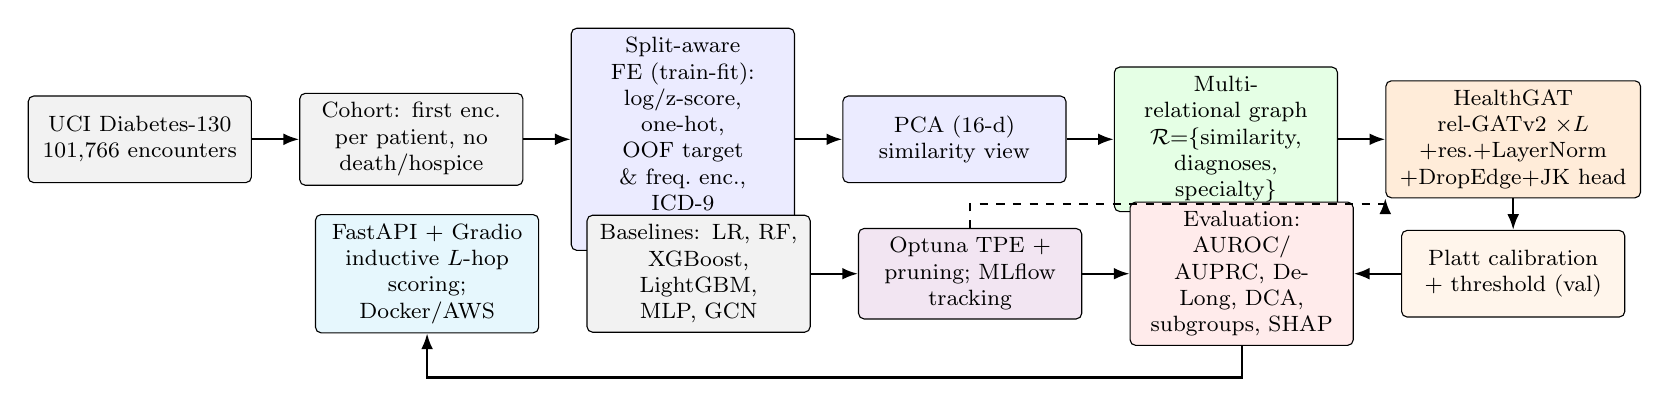
\begin{tikzpicture}[node distance=4mm and 6mm, font=\footnotesize,
  box/.style={draw, rounded corners=2pt, align=center, minimum height=11mm, text width=26mm, fill=#1},
  box/.default=white, arr/.style={-{Latex[length=2mm]}, thick}]
\node[box=gray!10] (raw) {UCI Diabetes-130\\101{,}766 encounters};
\node[box=gray!10, right=of raw] (coh) {Cohort: first enc.\\per patient, no\\death/hospice};
\node[box=blue!8, right=of coh] (fe) {Split-aware FE (train-fit):\\log/z-score, one-hot,\\OOF target \& freq.\ enc.,\\ICD-9 groups, codes};
\node[box=blue!8, right=of fe] (pca) {PCA (16-d)\\similarity view};
\node[box=green!10, right=of pca] (g) {Multi-relational graph\\$\mathcal{R}$=\{similarity,\\diagnoses, specialty\}};
\node[box=orange!15, right=of g, text width=30mm] (gat) {HealthGAT\\rel-GATv2 $\times L$\\+res.+LayerNorm\\+DropEdge+JK head};
\node[box=orange!8, below=of gat] (cal) {Platt calibration\\+ threshold (val)};
\node[box=red!8, left=of cal] (eval) {Evaluation: AUROC/\\AUPRC, DeLong, DCA,\\subgroups, SHAP};
\node[box=violet!10, left=of eval] (hpo) {Optuna TPE +\\pruning; MLflow\\tracking};
\node[box=gray!10, left=of hpo] (base) {Baselines: LR, RF,\\XGBoost, LightGBM,\\MLP, GCN};
\node[box=cyan!10, left=of base] (api) {FastAPI + Gradio\\inductive $L$-hop\\scoring; Docker/AWS};
\draw[arr] (raw)--(coh); \draw[arr] (coh)--(fe); \draw[arr] (fe)--(pca); \draw[arr] (pca)--(g);
\draw[arr] (g)--(gat); \draw[arr] (gat)--(cal); \draw[arr] (cal)--(eval);
\draw[arr] (hpo)--(eval); \draw[arr] (base)--(hpo); \draw[arr] (eval.south) |- ++(0,-4mm) -| (api.south);
\draw[arr, dashed] (hpo.north) -- ++(0,3mm) -| (gat.south west);
\end{tikzpicture}}
\caption{HealthGraph pipeline. Every fitted statistic (blue) uses training rows only; the same
fitted preprocessor and reference graph are reused at inference time.}
\label{fig:arch}
\end{figure*}

\subsection{Cohort and Preprocessing}
The target is $y{=}1$ if \texttt{readmitted}{=}``$<$30''. Our main cohort keeps the
\emph{first encounter per patient} and removes encounters ending in death or hospice (which
cannot be readmitted). This gives 69{,}973 patients with prevalence 9.0\%. Full-batch GAT
training on CPU limits the graph experiments to a stratified 20{,}000-patient subsample; the
tabular models are also evaluated on the full cohort (Sec.~\ref{sec:bench}). Splits are
stratified 70/15/15 (train/validation/test) and repeated over three seeds.

Feature engineering (Fig.~\ref{fig:arch}) is fitted on training rows only.
\textit{Numeric}: eight utilisation counts, with $\log(1{+}x)$ applied to heavy-tailed prior-visit
counts, plus engineered totals (prior visits, number of diabetes drugs, number of dose changes),
all z-scored.
\textit{Low-cardinality categoricals}: one-hot, with levels seen fewer than 20 times dropped.
\textit{High-cardinality}: the admitting specialty (72 levels) and three ICD-9 diagnoses
(700+ codes) get log-frequency encoding and smoothed target encoding
$\hat{\mu}_k = (\sum_{i\in k} y_i + m\,\bar{y})/(n_k + m)$ with $m{=}30$. This is computed
\emph{out-of-fold} (5 folds) for training rows, so no row sees its own label.
\textit{Domain grouping}: ICD-9 chapters following~\cite{strack2014}, as a primary-diagnosis
one-hot plus any-position counts. \textit{Codes}: multi-hot of the 100 most frequent 3-character
ICD-9 categories. In total this gives \nFeatures{} input features. Missing values (49\% of specialties,
and HbA1c not measured in 83\% of encounters) are kept as explicit categories, because the
absence of a measurement is itself informative.

\textbf{Dimensionality reduction.} PCA on the label-free numeric and one-hot block gives a
16-dimensional \emph{similarity view} (Fig.~\ref{fig:pca}) that keeps \pcaVar\% of the
variance. It is used to build edges, which avoids the curse of dimensionality in k-NN
search~\cite{vandermaaten2008}. t-SNE~\cite{vandermaaten2008} and UMAP~\cite{mcinnes2018}
project the learned embeddings for visual analysis.

\subsection{Multi-Relational Patient Graph}
Let $\mathcal{G}=(\mathcal{V},\mathcal{E},\mathcal{R})$ with one node per patient and three
relations: $r_1$, clinical similarity ($k_s$-NN, Euclidean, in the PCA space); $r_2$, shared
diagnoses ($k_c$-NN, cosine, on ICD multi-hot); and $r_3$, shared admitting specialty ($k_g$
random peers, a care-team proxy). Edges are symmetrised and de-duplicated per relation, and
self-loops get their own relation type. Because the edges use features only, the graph cannot
leak labels; the setting is transductive (test nodes are present without labels). We measure
\emph{outcome homophily} per relation as $P(y_j{=}1 \mid y_i{=}1, (j,i)\in r)$ and compare it
with the base rate.

\subsection{HealthGAT}
An encoder maps $\mathbf{x}_i$ to $\mathbf{h}^{(0)}_i=\mathrm{ELU}(\mathbf{W}_0\mathbf{x}_i)$.
Each relation-aware GATv2 layer computes, per head $h$,
\begin{align}
e^{h}_{ij} &= \mathbf{a}_h^{\top}\,\mathrm{LeakyReLU}\big(\mathbf{W}^h_s\mathbf{h}_j+\mathbf{W}^h_t\mathbf{h}_i+\mathbf{r}^h_{\tau(j,i)}\big),\\
\alpha^h_{ij} &= \frac{\exp(e^h_{ij})}{\sum_{k\in\mathcal{N}(i)\cup\{i\}}\exp(e^h_{ik})},\quad
\mathbf{m}_i=\big\Vert_{h}\sum_{j}\alpha^h_{ij}\mathbf{W}^h_s\mathbf{h}_j,
\end{align}
where $\mathbf{r}_{\tau}$ is a learned embedding of the edge's relation. It lets each head
weigh similarity, diagnosis and specialty neighbours differently, at far fewer parameters than
R-GCN's per-relation weight matrices~\cite{schlichtkrull2018}. Applying the non-linearity before
$\mathbf{a}_h$ gives dynamic attention~\cite{brody2022}. Each layer uses a residual connection,
LayerNorm and dropout: $\mathbf{h}^{(\ell+1)}=\mathrm{LN}(\mathbf{h}^{(\ell)}+\mathrm{Drop}(\mathrm{ELU}(\mathbf{m})))$.
A jumping-knowledge head maps $[\mathbf{h}^{(0)}\Vert\mathbf{h}^{(L)}]$ through an MLP to a
logit $z_i$. Training minimises class-weighted binary cross-entropy (positive weight
$(1-\bar y)/\bar y$) with AdamW, gradient clipping, DropEdge~\cite{rong2020} and
ReduceLROnPlateau, and stops early on validation AUPRC. The edge softmax is implemented with
scatter operations, so the model needs no graph library.

\textbf{Calibration and decisions.} The class weighting shifts all logits upward. Temperature
scaling~\cite{guo2017} can only rescale them, so we fit Platt scaling~\cite{platt1999}
$p=\sigma(az+b)$ on the validation split. The operating threshold maximises validation F1 and
is applied unchanged to the test set.

\subsection{Hyperparameter Search and Experiment Tracking}
Optuna~\cite{akiba2019} with a TPE sampler maximises validation AUPRC on the seed-0 split. For
HealthGAT the search space covers hidden size $\{16,32\}$, heads $\{2,4\}$, layers $\{1,2,3\}$,
dropout $[0.2,0.6]$, DropEdge $[0,0.4]$, learning rate $[3{\times}10^{-4},5{\times}10^{-3}]$
(log), weight decay $[10^{-4},2{\times}10^{-2}]$ (log), and the \emph{graph density}
$k_s\in\{5,10,20\}$, $k_c\in\{3,5,10\}$, $k_g\in\{0,4,8\}$, with median pruning after 30
epochs. XGBoost, LightGBM and RF get their own TPE studies; logistic regression uses an
exhaustive grid over $C$. The test split is never used for any selection. Every trial,
per-epoch curve, metric and figure is logged to MLflow~\cite{zaharia2018} (SQLite backend) and
mirrored to a JSONL log.

\subsection{Evaluation}
We report AUROC, AUPRC (the primary metric, given 9\% prevalence), log-loss, Brier score,
expected calibration error (ECE), F1, sensitivity, specificity, PPV and top-decile capture. All
are given as mean$\pm$sd over three seeds, with 1{,}000-sample bootstrap 95\% CIs. AUROC
differences use the paired DeLong test~\cite{delong1988,sun2014}, and decisions at the tuned
threshold use McNemar's test. Clinical utility uses decision-curve analysis~\cite{vickers2006}.
Interpretability uses SHAP~\cite{lundberg2017} for the tree baseline, gradient$\times$input for
HealthGAT, attention budgets per relation, and a relation ablation.

%% ------------------------------------------------------------------
\section{Implementation and Experiments}
\textbf{Environment.} AMD Ryzen 7 7445HS (6 cores / 12 threads), 15\,GB RAM, no GPU; Windows 11;
Python 3.14, PyTorch 2.14 (CPU), scikit-learn 1.8, XGBoost 3.2, LightGBM 4.6, Optuna 5.0,
MLflow 3.17, SHAP 0.52. All models train full-batch on CPU.

\textbf{Workflow.} The pipeline is a Python package driven by YAML configs
(\texttt{python -m healthgraph all}). Its stages are \texttt{tune}, \texttt{experiment},
\texttt{ablation}, \texttt{analyze} and \texttt{benchmark}, and each one resumes from
checkpoints (Optuna's SQLite store and per-run result files), so interrupted runs continue
where they stopped. Each seed re-fits the preprocessor and
rebuilds the graph on that seed's training split. Twenty-two pytest tests check the layer
mathematics (edge-softmax normalisation, locality of message passing), the exactness of
inductive inference, and the API contract.

\textbf{Tuning outcome.} The HealthGAT study ran \nTrials{} trials (\nComplete{} completed,
\nPruned{} pruned by the median rule, \nInterrupted{} lost to process interruptions). The best
configuration (validation AUPRC \bestValAuprc) uses \besthidden{} hidden units $\times$
\bestheads{} heads, \bestlayers{} layers, dropout \bestdropout, DropEdge \bestedgedropout,
learning rate \bestlr{} and weight decay \bestweightdecay, with graph density $k_s{=}\bestKsim$,
$k_c{=}\bestKcode$, $k_g{=}\bestKgroup$ (Fig.~\ref{fig:optuna}). MLP and GCN share the tuned
GNN configuration, so they differ from HealthGAT only in their aggregation. The tuned graph has
\nEdges{} directed edges over \nRef{} patients.

\begin{figure}[t]\centering
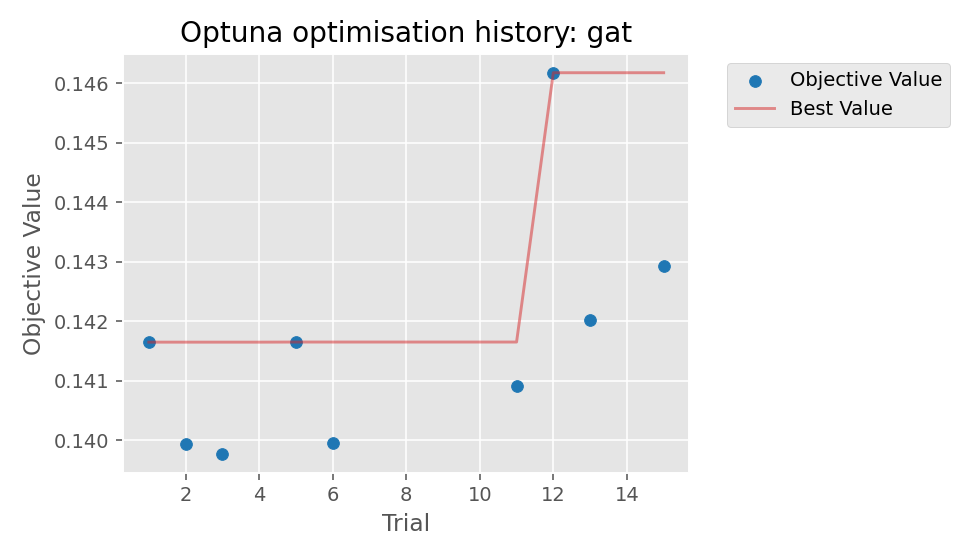
\includegraphics[width=0.49\columnwidth]{history_gat.png}\hfill
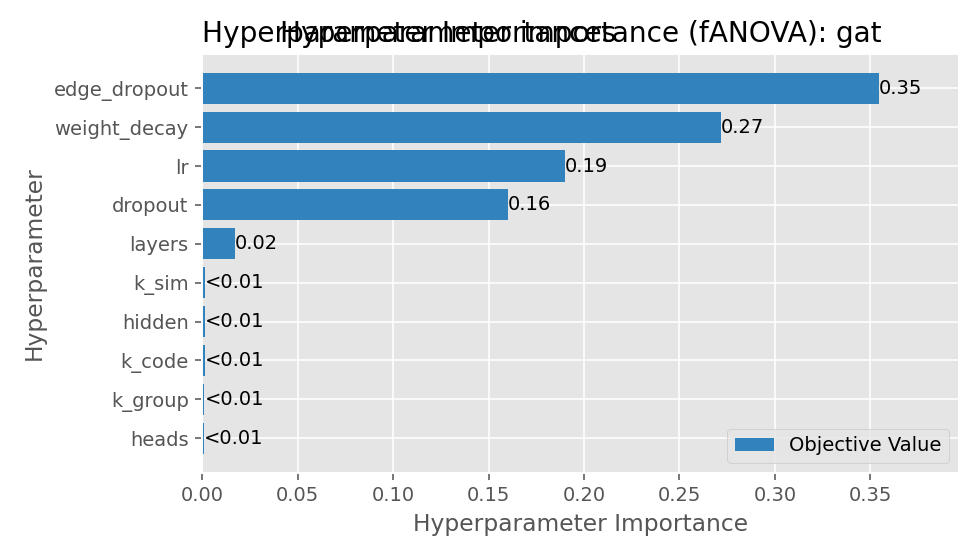
\includegraphics[width=0.49\columnwidth]{importance_gat.png}
\caption{Optuna search for HealthGAT: optimisation history (left) and fANOVA hyperparameter
importance (right).}\label{fig:optuna}
\end{figure}

\begin{figure*}[t]\centering
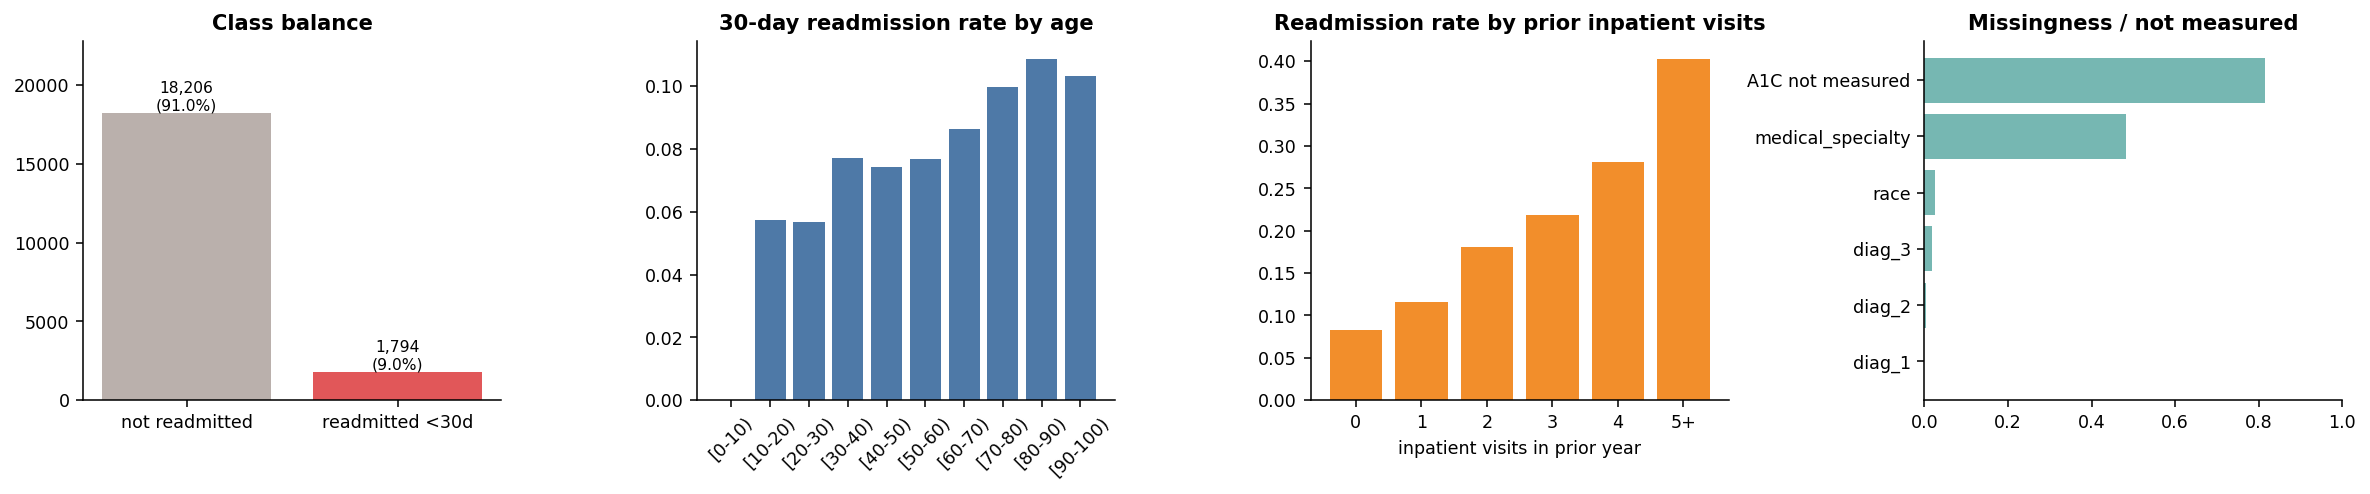
\includegraphics[width=\textwidth]{eda.png}
\caption{Exploratory analysis of the 20k-patient cohort: 9.0\% prevalence; readmission rises with
age and steeply with prior inpatient stays; HbA1c is not measured in most encounters and the
specialty is missing for about half.}\label{fig:eda}
\end{figure*}

\begin{figure}[t]\centering
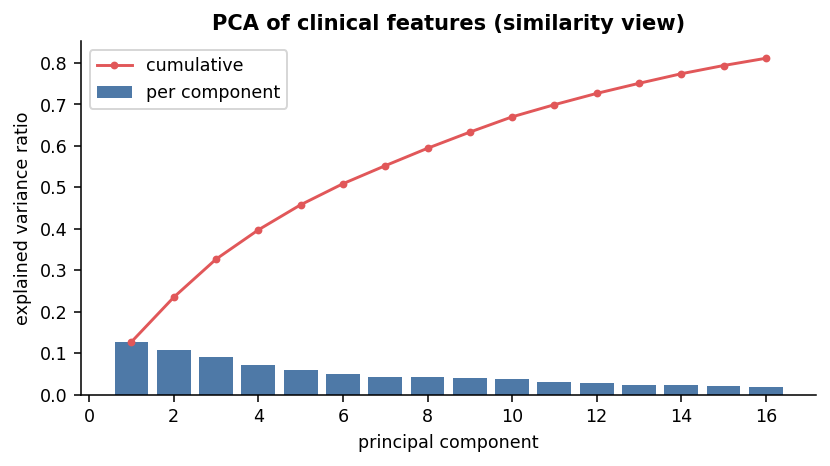
\includegraphics[width=0.49\columnwidth]{pca_variance.png}\hfill
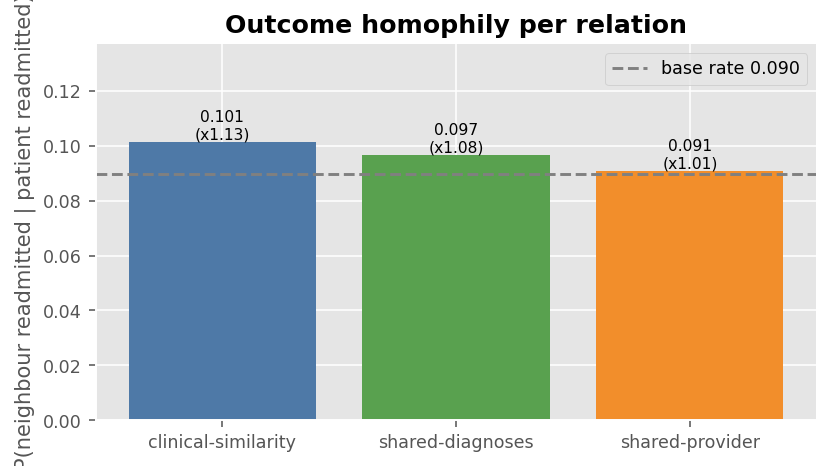
\includegraphics[width=0.49\columnwidth]{homophily.png}
\caption{Left: PCA spectrum of the similarity view. Right: outcome homophily per relation:
the probability that a readmitted patient's neighbour is also readmitted, against the
\prevalence\% base rate.}\label{fig:pca}
\end{figure}

\begin{figure*}[t]\centering
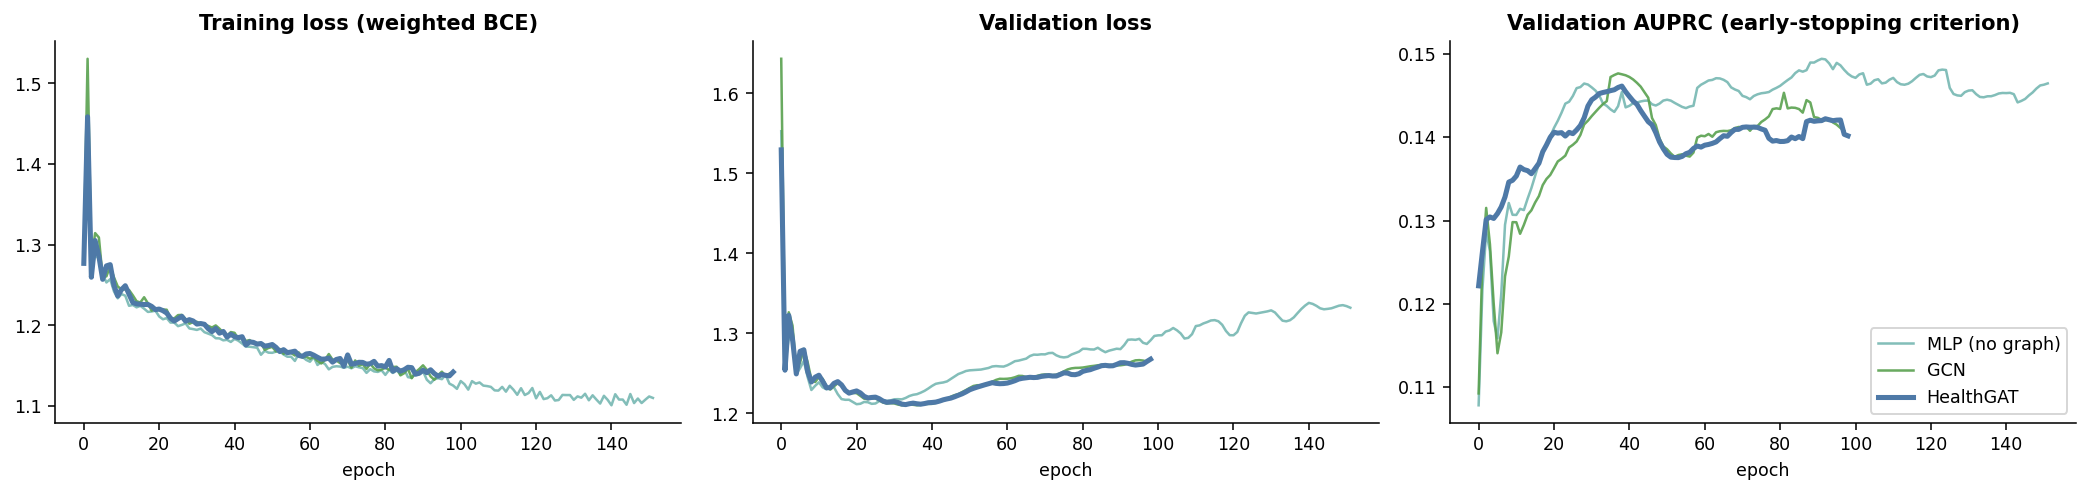
\includegraphics[width=\textwidth]{training_curves.png}
\caption{Training dynamics (seed 0): training loss, validation loss and validation AUPRC (the
early-stopping criterion). The graph models converge in fewer epochs than the MLP.}\label{fig:curves}
\end{figure*}

%% ------------------------------------------------------------------
\section{Results and Comparative Analysis}
\inputtable{main_results}

\subsection{Discrimination, Calibration and Significance}
Table~\ref{tab:main} gives test-set results on the strict cohort. All seven models land in a
narrow band, AUROC \aurocXGB--\aurocLR. The best AUROC is logistic regression's
(\aurocLR$\pm$\aurocsdLR), with the MLP (\aurocMLP), GCN (\aurocGCN) and HealthGAT
(\aurocGAT$\pm$\aurocsdGAT) close behind. Random forest has the best AUPRC (\auprcRF). The
seed-to-seed spread (sd $\approx$0.02--0.03) is as large as the gaps between models: seed~1 is
about 0.04 harder for \emph{every} model. The paired DeLong tests (Table~\ref{tab:sig}) find no
significant difference between HealthGAT and any baseline in any seed, apart from a single
borderline $p{=}0.047$ against the MLP in seed~2, which is expected by chance across 18 tests.
Tuned XGBoost had the highest \emph{validation} AUPRC during tuning, yet the lowest test AUROC
(\aurocXGB). Tuning on a single split clearly overfits that split, which is a caution for
leaderboard-style comparisons.

After Platt scaling every model is well calibrated (ECE $\le$0.006,
Fig.~\ref{fig:roc}). At the validation-tuned threshold HealthGAT flags \sensGAT\% of
readmissions with PPV \ppvGAT\%, about 1.5$\times$ the base rate, and its top risk decile
captures \topdecGAT\% of all readmissions. The decision curve (Fig.~\ref{fig:dca}) shows a
positive net benefit over ``treat all'' for threshold probabilities between roughly 5\% and 20\%,
the range relevant to low-cost interventions such as follow-up calls.

\inputtable{significance}

\begin{figure*}[t]\centering
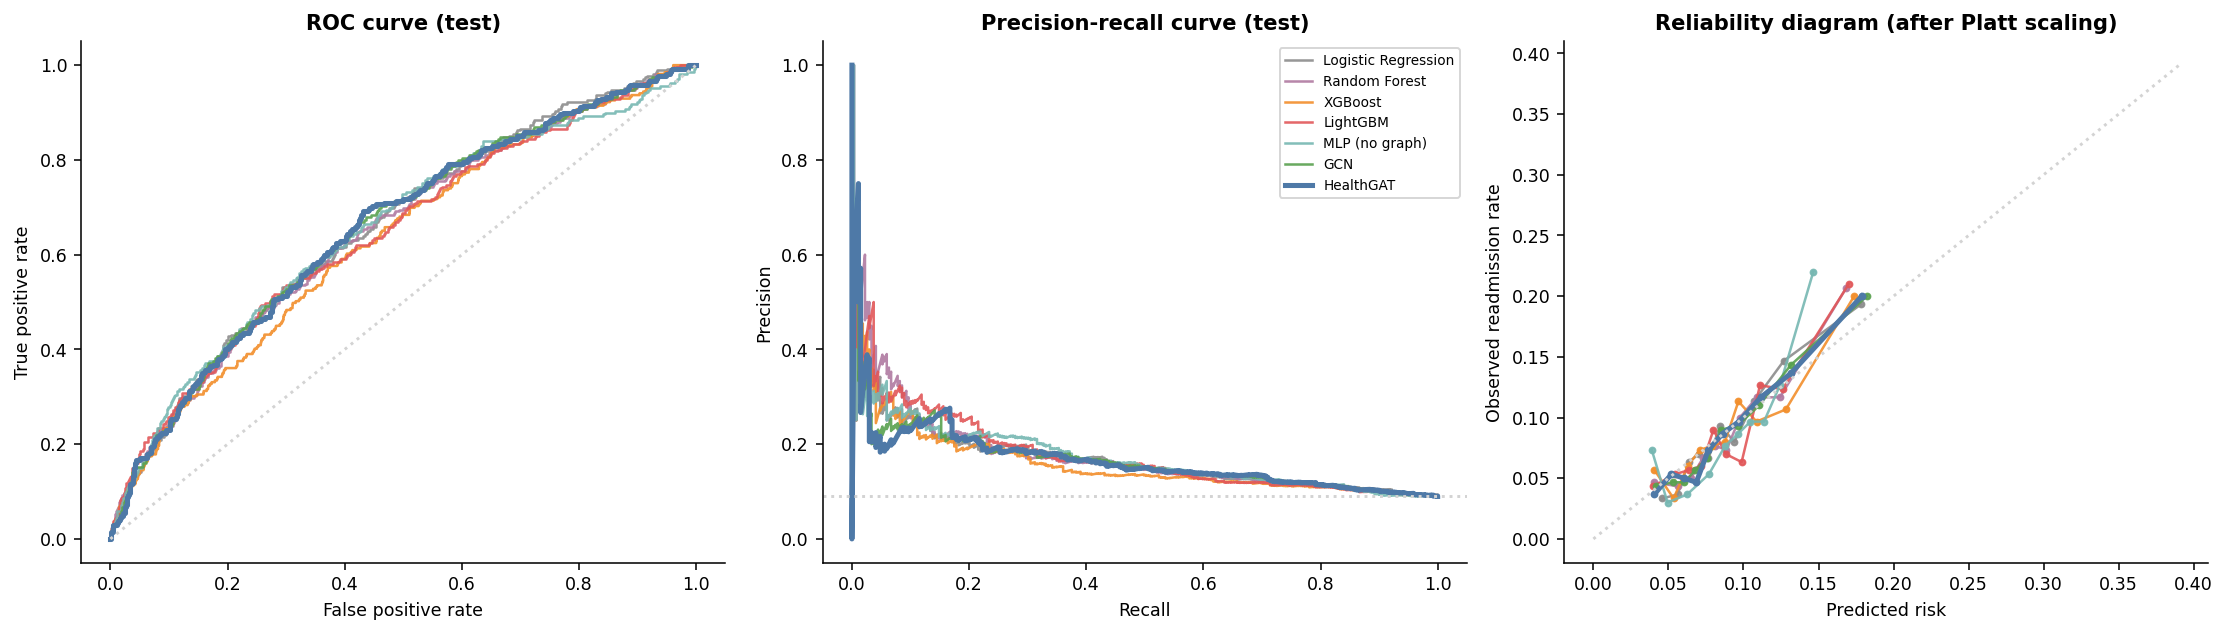
\includegraphics[width=\textwidth]{roc_pr_calibration.png}
\caption{Seed-0 test set: ROC (left), precision--recall (middle) and reliability diagram after
Platt scaling (right). The curves of all models overlap closely.}\label{fig:roc}
\end{figure*}

\begin{figure}[t]\centering
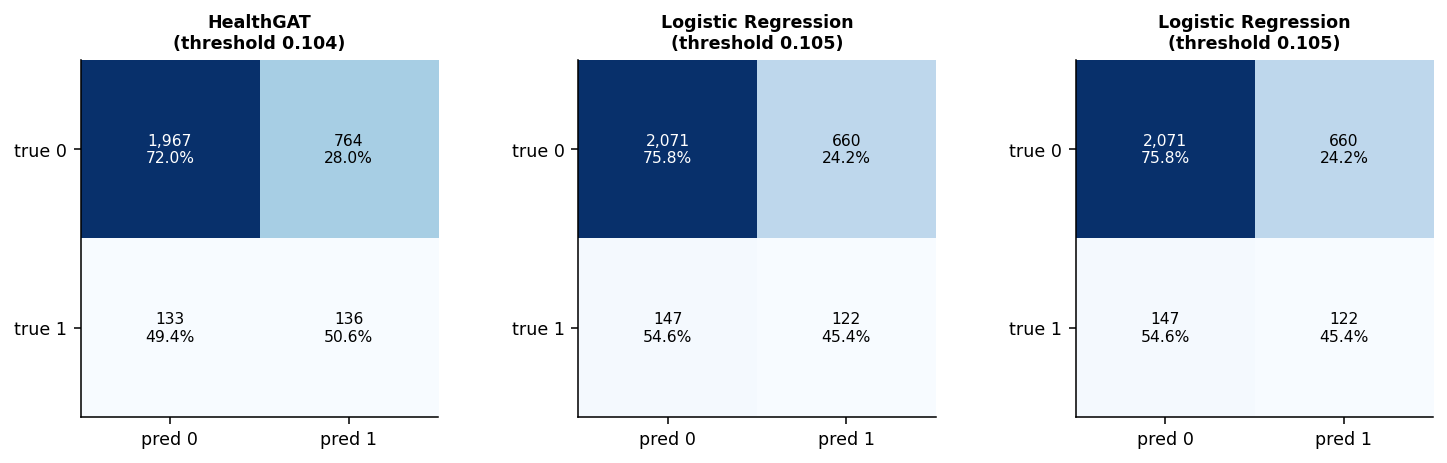
\includegraphics[width=\columnwidth]{confusion_matrices.png}
\caption{Confusion matrices at validation-tuned (max-F1) thresholds, seed-0 test set.}\label{fig:cm}
\end{figure}

\subsection{Comparison with Published Benchmarks}\label{sec:bench}
Published numbers are not directly comparable to ours, because the two studies use all
encounters with encounter-level splits~\cite{emijohnson2025,salim2026}. We therefore re-ran our
tuned tabular models under four protocols (Table~\ref{tab:bench}). Under the published protocol
(P1, \benchNPOne{} encounters) our XGBoost reaches \benchPOneXGB{} and logistic regression
\benchPOneLR, matching or exceeding the best published results (0.667 and 0.664--0.665). This
confirms that the pipeline is competitive. Removing same-patient leakage with a patient-grouped
split (P2; under P1 \benchOverlapPOne{} test patients also appear in training) changes AUROC only
slightly (\benchPTwoXGB{} for XGBoost). The cohort definition matters much more: restricting to
first encounters and excluding death and hospice (P3) lowers AUROC to \benchPThreeXGB{}--%
\benchPThreeLGBM. The reason is that later encounters of frequently readmitted patients, which
carry rich utilisation history, are removed. Sample size matters too: the 20k-patient graph
cohort (P4) costs the tabular models a further 0.01--0.03 against the full 70k (P3). On P4,
logistic regression gives \benchPFourLR{} (identical to Table~\ref{tab:main}, a consistency
check) against \aurocGAT{} for HealthGAT on the same splits. Cohort definition, not model
choice, explains most of the spread in published AUROCs.

\inputtable{benchmark}

\subsection{Why the Graph Does Not Help Here, and When It Does}
\textbf{Homophily.} Fig.~\ref{fig:pca} (right) shows the outcome signal carried by each
relation. A readmitted patient's clinical-similarity neighbour is readmitted \homSim{} of the
time (\homLiftSim$\times$ the base rate), a diagnosis neighbour \homDx{}
(\homLiftDx$\times$) and a same-specialty neighbour \homSpec{} (\homLiftSpec$\times$). The
graph is barely more homophilous than random, and much of the signal it does carry (clinical
similarity) is already in each node's own features. Message passing then has little to add, and
can even dilute a node's own evidence~\cite{zhu2020}.

\textbf{Ablation and attention.} Retraining HealthGAT without each relation
(Table~\ref{tab:abl}, Fig.~\ref{fig:abl}) changes AUROC by less than the seed-to-seed spread
(all relations \ablAll; self-loops only \ablNoEdges). Removing \emph{only} the clinical-similarity
edges was slightly worse in all three seeds (\ablNoSim), whereas removing every edge was not.
This suggests the similarity edges mainly offset noise that the diagnosis and specialty edges
introduce, rather than adding signal of their own. The learned attention matches this.
HealthGAT gives \attSim\% of its attention to clinical-similarity neighbours, \attDx\% to
diagnosis neighbours and \attSpec\% to specialty neighbours, and its attention lift towards
neighbours who were later readmitted is only \attLiftPos{} (1.00 = uniform).

\textbf{Controlled synthetic study.} To check that HealthGAT can exploit a graph when one is
informative, we generated 6{,}000 synthetic patients with eight latent phenotypes and 120
providers whose hidden quality affects the outcome. The provider leaves only noisy traces in
individual records (length of stay, polypharmacy, follow-up), and same-provider edges carry
\synHomLiftSpec$\times$ outcome enrichment. Here the graph models clearly beat every tabular
model (Table~\ref{tab:syn}): HealthGAT reaches \synGAT{} against \synMLP{} for the identical
network without message passing and \synLGBM{} for LightGBM, with DeLong $p<0.01$ in two of the
three seeds. That closes about a third of the gap to the oracle (\synOracle), which uses the
true risk. Removing provider edges is the most costly ablation
(\synablAll{}~$\rightarrow$~\synablNoSpec), about as costly as removing every edge
(\synablNoEdges), while dropping the other two relations slightly \emph{helps}. HealthGAT and GCN
are again within noise of each other (\synGAT{} against \synGCN), so in this setting the gain
comes from message passing over the right relation more than from attention itself. The architecture therefore works; whether
it helps depends on whether the graph carries outcome signal not already in the node features.
This can be checked cheaply \emph{before} training, using the homophily diagnostic.

\inputtable{ablation}
\inputtable{synthetic}

\begin{figure}[t]\centering
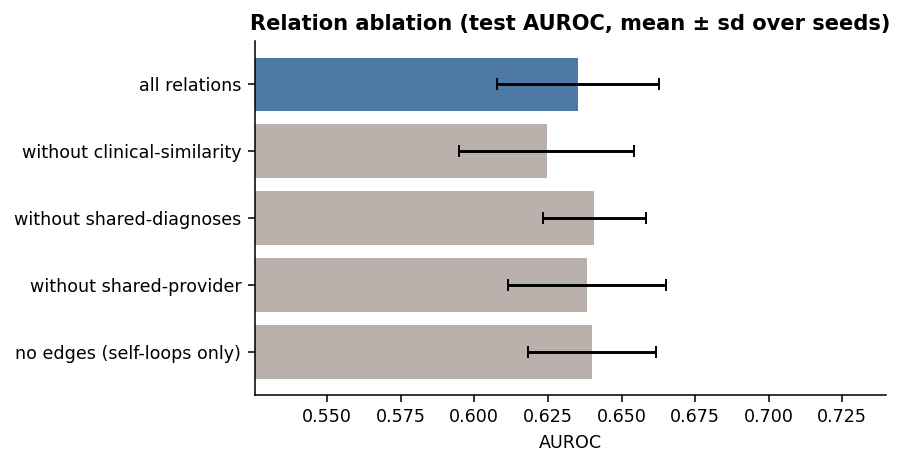
\includegraphics[width=\columnwidth]{ablation.png}
\caption{Relation ablation on UCI (test AUROC, mean$\pm$sd over seeds).}\label{fig:abl}
\end{figure}

\subsection{Interpretability}
SHAP for \shapModel{} (Fig.~\ref{fig:shap}) and gradient$\times$input for HealthGAT rank the
same drivers at the top: prior inpatient stays, discharge home (protective), length of stay,
discharge to skilled nursing or rehabilitation, and the engineered diagnosis target and
frequency encodings. This confirms the value of the high-cardinality encodings. The embedding
projections (Fig.~\ref{fig:emb}) show HealthGAT ordering patients along a risk axis that is not
visible in the raw features.

\begin{figure}[t]\centering
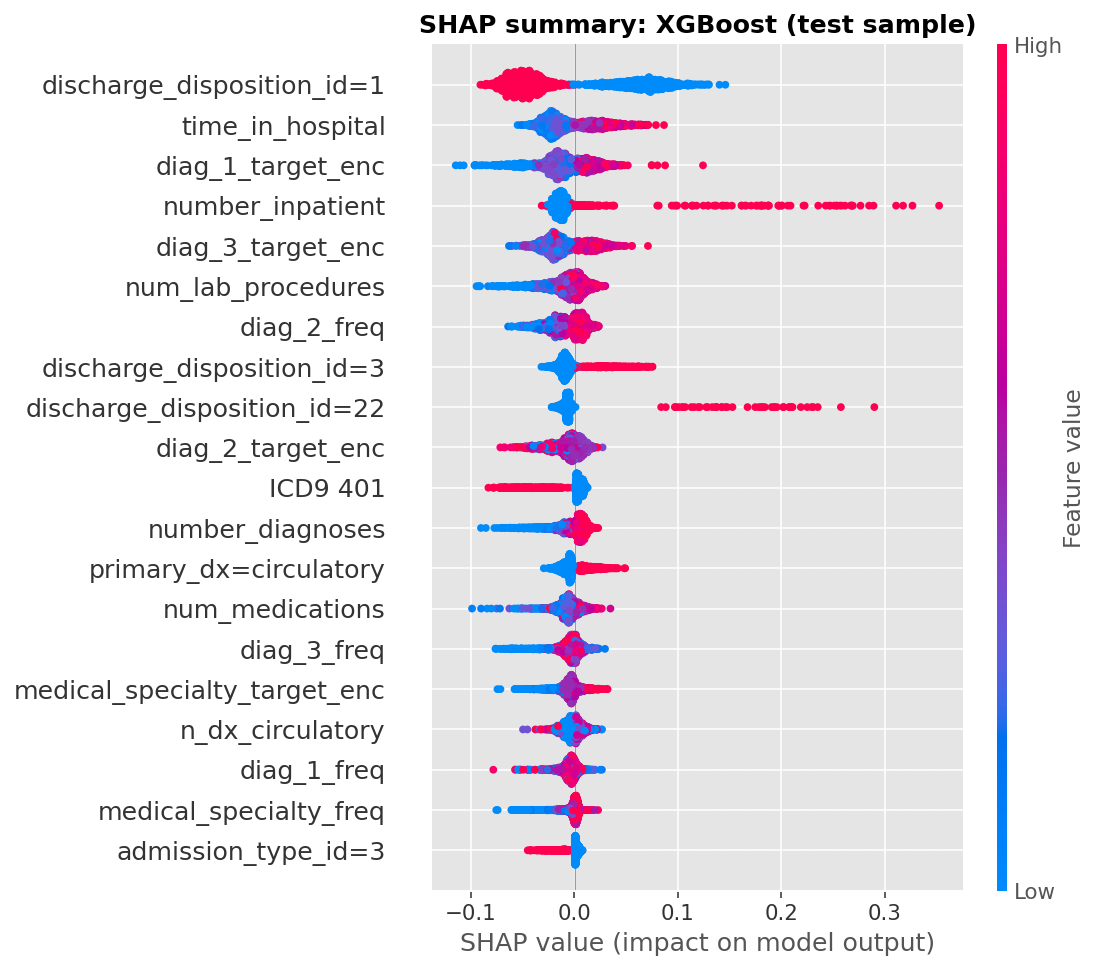
\includegraphics[width=\columnwidth]{shap_tree_model.png}
\caption{SHAP summary for \shapModel{} (2{,}000 seed-0 test patients).}\label{fig:shap}
\end{figure}

\begin{figure*}[t]\centering
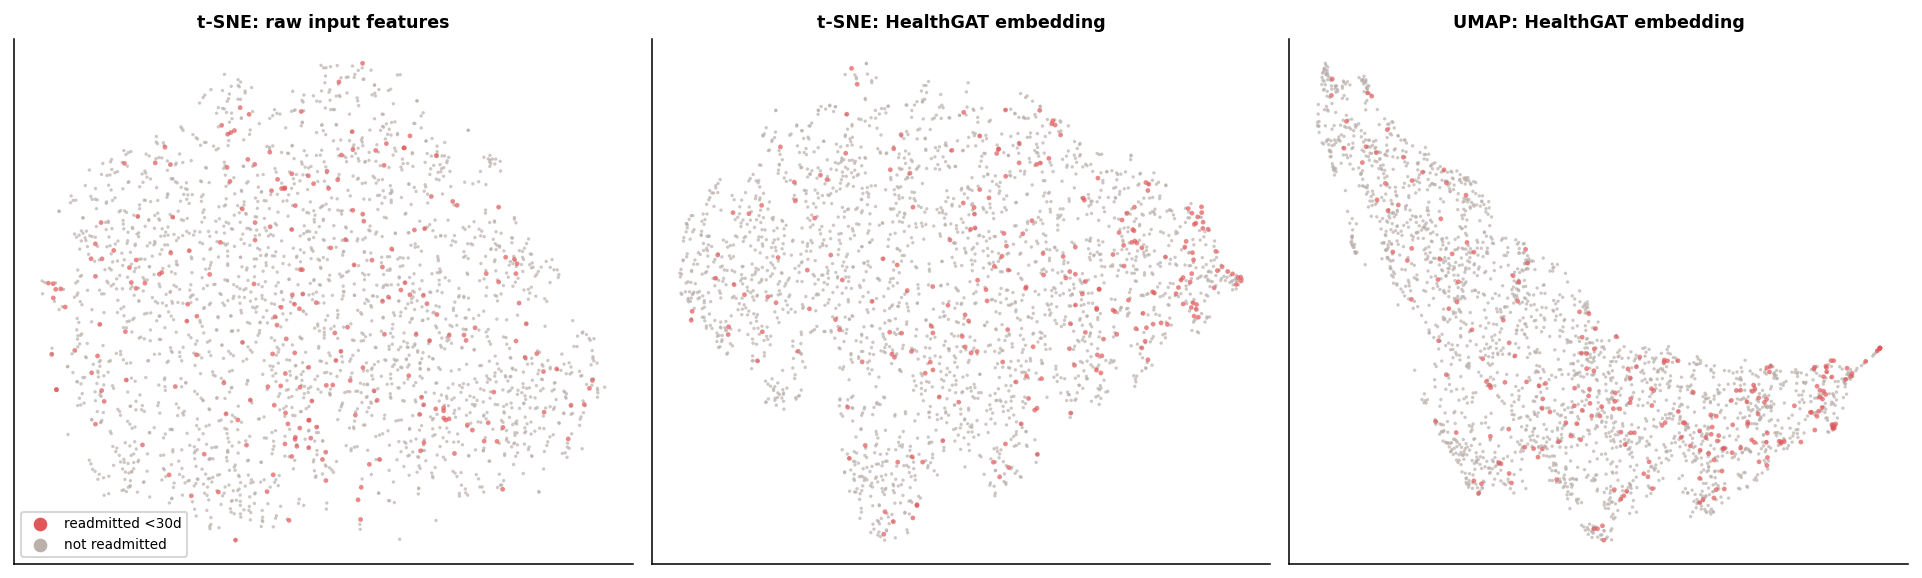
\includegraphics[width=0.92\textwidth]{embeddings.png}
\caption{t-SNE of raw input features against t-SNE and UMAP of the learned HealthGAT
representation (2{,}500 test patients; red = readmitted).}\label{fig:emb}
\end{figure*}

\subsection{Error Analysis}
\textbf{Subgroups} (Fig.~\ref{fig:sub}, test sets pooled over seeds). Calibration holds in every
subgroup (largest gap \subMaxCalGap{} percentage points), and discrimination is similar for women
and men and for Caucasian and African-American patients. Performance is weakest
\emph{within} patients who already have prior inpatient stays (AUROC \subWorstAuc{} for
\subWorst). Prior utilisation dominates the score, so once it is fixed the remaining features
separate risk poorly, and the model under-predicts risk for the most frequent re-admitters.

\textbf{Error profile.} False negatives (\errFNN) look like true negatives: they average
\errFNInp{} prior inpatient stays, against \errTPInp{} for true positives, with a mean predicted
risk of \errFNRisk\%. The model mostly misses \emph{first} readmissions that lack any utilisation
history. False positives (\errFPN) are patients with prior stays (\errFPInp{} on average) who
were not readmitted. Both failure modes point to the same missing information: social factors,
post-discharge care and medication adherence, none of which Diabetes-130 records.

\begin{figure*}[t]\centering
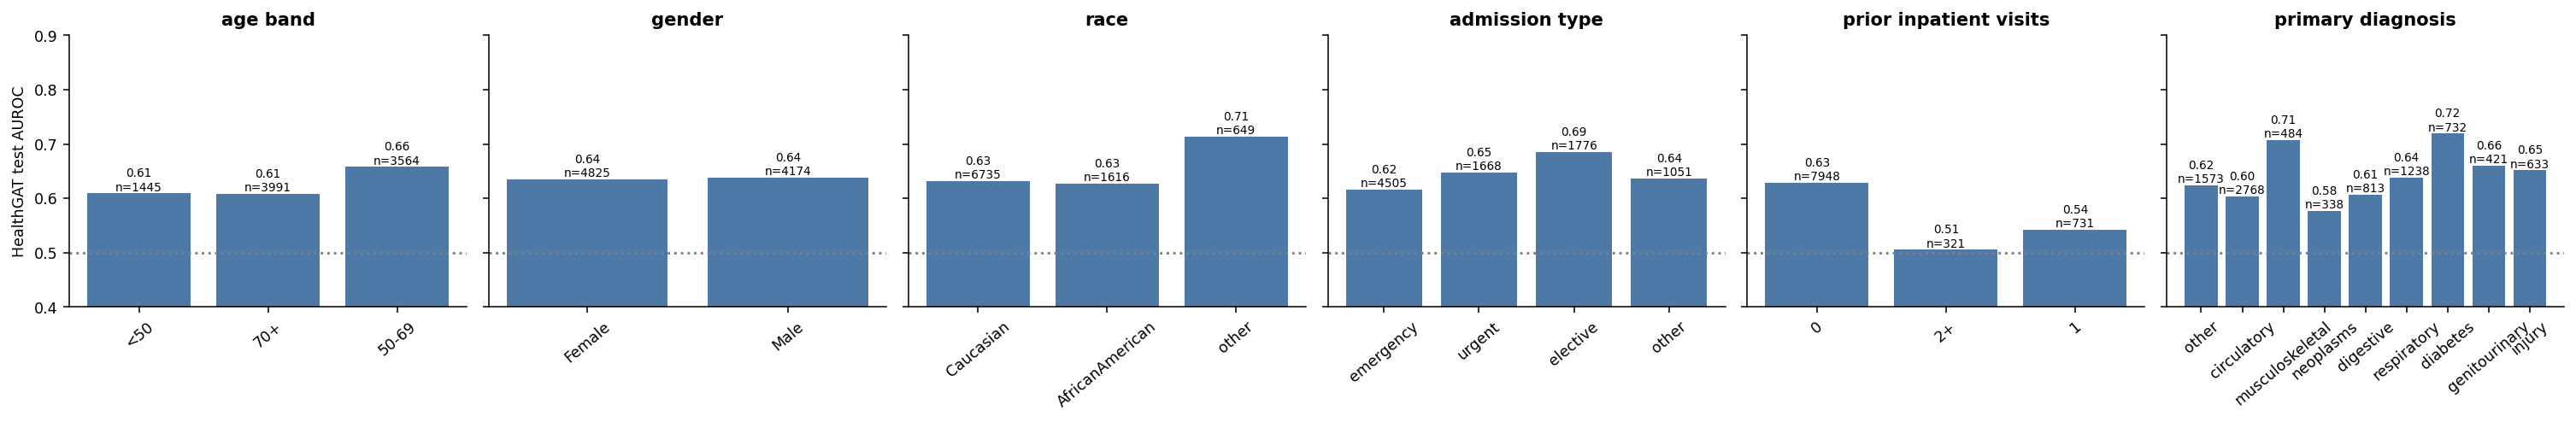
\includegraphics[width=\textwidth]{subgroups.png}
\caption{HealthGAT test AUROC by subgroup (test sets pooled over seeds; $n$ per bar; dotted line = chance).}\label{fig:sub}
\end{figure*}

\begin{figure}[t]\centering
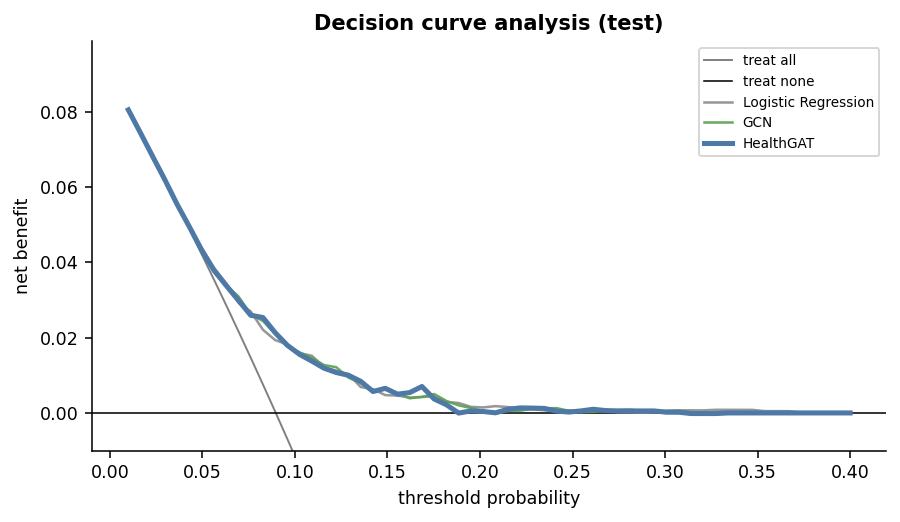
\includegraphics[width=\columnwidth]{decision_curve.png}
\caption{Decision-curve analysis: net benefit against threshold probability.}\label{fig:dca}
\end{figure}

%% ------------------------------------------------------------------
\section{Deployment}
\textbf{Inductive inference.} A GNN trained transductively must score patients it has never
seen. The deployment bundle (\texttt{artifacts/healthgat\_uci.pt}, 35\,MB) stores the fitted
preprocessor, the reference cohort's features and edges, the model weights, the Platt
parameters and the decision threshold. A new encounter is preprocessed with the \emph{same}
fitted transform and attached to the reference graph with the training rules: $k_s$ nearest
neighbours in PCA space, $k_c$ cosine neighbours on its ICD codes, and $k_g$ same-specialty
peers drawn with a seed derived from the request, so identical requests get identical edges.
An $L$-layer GNN's output depends only on the node's $L$-hop in-neighbourhood, so we extract
that subgraph from a CSR index and run the forward pass on it alone. A unit test checks that
the result equals a full-graph pass on the augmented graph to within $10^{-4}$. With the tuned
$L{=}3$ the subgraph covers about 10k nodes, and scoring takes about 0.3\,s per request on CPU
(0.5\,s with explanations).

\textbf{Local API.} A FastAPI service exposes \texttt{POST /predict}, \texttt{POST /predict/batch}
(at most 100), \texttt{GET /model/info} and \texttt{GET /health}, with auto-generated OpenAPI
documentation at \texttt{/docs}. Pydantic schemas enforce input validation: enumerated age
bands and categorical codes, numeric ranges taken from the data dictionary (e.g.\ length of stay
1--14 days), an ICD-9 format regex, rejection of unknown fields, and a domain rule that refuses
patients who died or were discharged to hospice. Invalid requests receive HTTP 422 with a
per-field explanation. Each response contains the calibrated risk, a risk band, the follow-up
flag, the top gradient-based risk drivers and the most-attended similar past patients, which
serves as a case-based explanation. Middleware adds request IDs and timing headers, and logs
every call.

\textbf{Container and cloud.} A Gradio UI (Fig.~\ref{fig:ui}) is mounted at \texttt{/ui} in the
same process. The
Docker image (\texttt{python:3.12-slim}, CPU PyTorch, pinned dependencies, non-root UID 1000,
port 7860, health check; 2.15\,GB) was built and tested locally (health check passing, valid
predictions, 422 on invalid input). It is deployed on \textbf{AWS EC2} (free-tier t3.micro,
Amazon Linux 2023, ap-south-1) by one script (\texttt{deploy/deploy\_aws\_ec2.sh}). The script
uploads the build context to a private S3 bucket and creates a security group that opens only
HTTP. The instance's first-boot script adds 2\,GB of swap (the service needs about 0.6\,GB of the
instance's 1\,GB RAM), installs Docker, builds the image and runs it with automatic restart. The
live service returns the same prediction as the local container, in about 0.4\,s per request.
Live UI: \url{http://15.252.73.160/ui}; API documentation: \url{http://15.252.73.160/docs}.
A Hugging Face Spaces configuration is also provided, since Docker Spaces now require a paid plan.

\begin{figure*}[t]\centering
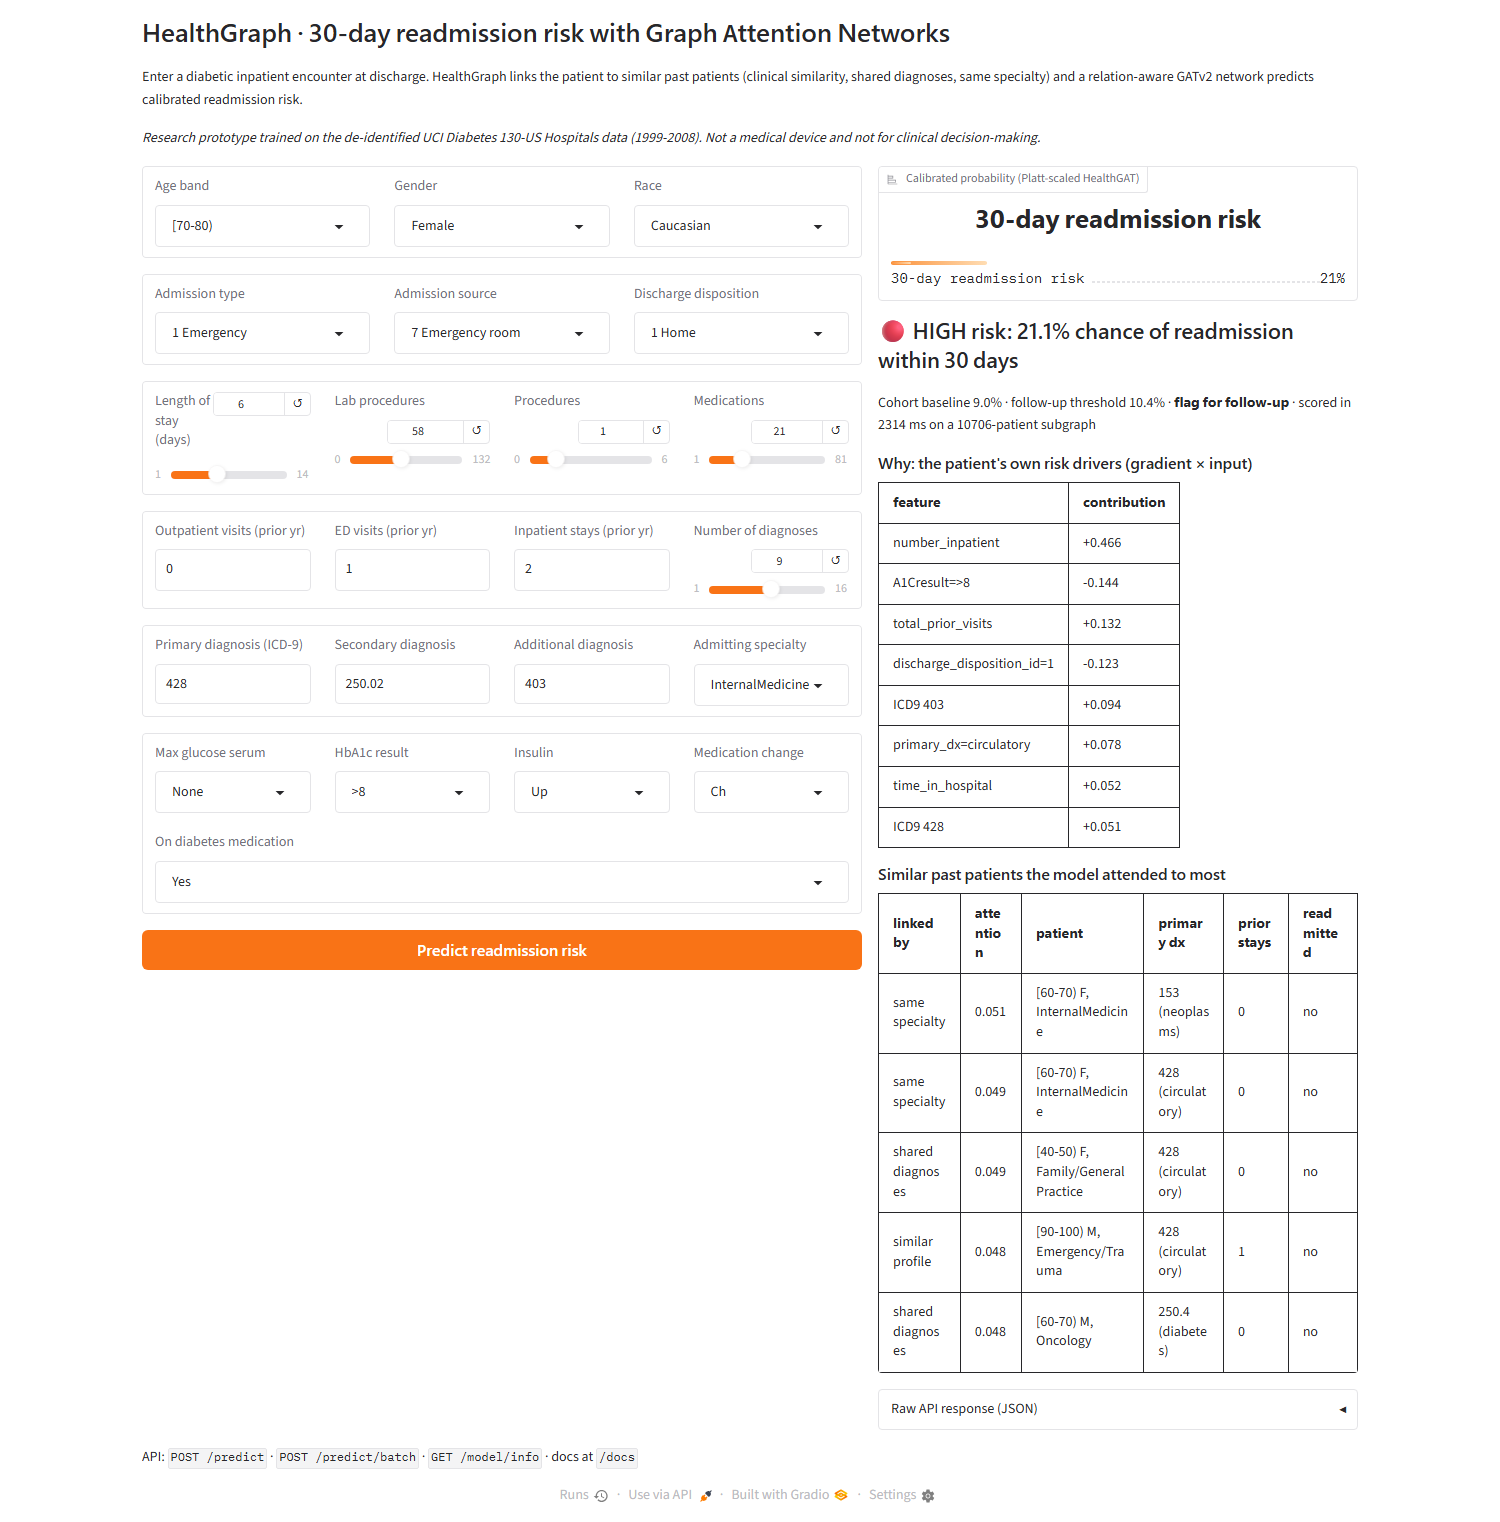
\includegraphics[width=0.78\textwidth]{ui_screenshot.png}
\caption{HealthGraph web UI (Gradio, served at \texttt{/ui} by the FastAPI app): the encounter form
(left) and the response (right), showing the calibrated risk and band, the patient's own risk
drivers, and the most-attended similar past patients with the relation that links them. The
nearly uniform attention weights ($\approx$0.05) match the finding that no neighbour stands out
on this data.}\label{fig:ui}
\end{figure*}

%% ------------------------------------------------------------------
\section{Conclusion and Future Scope}
We built HealthGraph, an end-to-end system for 30-day readmission risk built around a
relation-aware GATv2 network over a multi-relational patient graph. It covers leakage-safe
feature engineering, automated Optuna tuning, MLflow tracking, a protocol-controlled benchmark
and a validated, containerised deployment. Under the published evaluation protocol our pipeline
matches or exceeds the best reported AUROC on Diabetes-130 (\benchPOneXGB{} against 0.667).

The central finding is a nuanced one. On the real data, HealthGAT is as accurate and well
calibrated as strong tabular baselines but not significantly better
(\aurocGAT{} against \aurocLR{} for logistic regression). Its patient graph is only weakly
outcome-homophilous (\homLiftSim$\times$ the base rate at best), and the ablation, the attention
budgets and the controlled synthetic study all tell the same story: patient graphs help when
they encode latent shared factors that individual records do not show (on synthetic data
\synGAT{} against \synMLP), and add nothing otherwise. Two practical lessons follow. Measure
homophily before committing to a GNN, and report results under an explicit cohort definition,
because cohort choice moved AUROC more than any model did.

\textbf{Deployment considerations.} The model must be recalibrated, and its reference graph
refreshed, for each new site and time period: the data is from 1999--2008, uses ICD-9, and has
no post-discharge information. Scoring cost grows with $L$ (the subgraph grows roughly geometrically with depth). Three-layer
configurations led the search by only 0.004 validation AUPRC (0.146 against 0.142), so a
2-layer model is a reasonable trade-off when latency matters.

\textbf{Future scope.} (i)~Richer, more homophilous relations, such as true provider or ward
identifiers, shared medications or temporal encounter chains in MIMIC-IV; (ii)~heterophily-aware
or label-propagation variants~\cite{zhu2020}; (iii)~mini-batch neighbour sampling to train on the
full 70k cohort and beyond; and (iv)~prospective validation together with fairness auditing across
subgroups.

%% ------------------------------------------------------------------
\begin{thebibliography}{99}\footnotesize
\bibitem{strack2014} B.~Strack, J.~P. DeShazo, C.~Gennings, J.~L. Olmo, S.~Ventura, K.~J. Cios, and J.~N. Clore, ``Impact of HbA1c measurement on hospital readmission rates: Analysis of 70,000 clinical database patient records,'' \emph{BioMed Research International}, vol.~2014, Art.~no.~781670, 2014.
\bibitem{emijohnson2025} O.~G. Emi-Johnson and K.~J. Nkrumah, ``Predicting 30-day hospital readmission in patients with diabetes using machine learning on electronic health record data,'' \emph{Cureus}, vol.~17, no.~4, Art.~no.~e82437, 2025.
\bibitem{salim2026} S.~S. Salim and A.~A. Ibrahim, ``A machine learning approach for predicting 30-day hospital readmission in patients with diabetes,'' \emph{Healthcare}, vol.~14, no.~9, Art.~no.~1185, 2026.
\bibitem{tang2023} S.~Tang, A.~Tariq, J.~A. Dunnmon, U.~Sharma, P.~Elugunti, D.~L. Rubin, B.~N. Patel, and I.~Banerjee, ``Predicting 30-day all-cause hospital readmission using multimodal spatiotemporal graph neural networks,'' \emph{IEEE J. Biomed. Health Inform.}, vol.~27, no.~4, pp.~2071--2082, 2023.
\bibitem{vanwalraven2010} C.~van Walraven \emph{et al.}, ``Derivation and validation of an index to predict early death or unplanned readmission after discharge from hospital to the community,'' \emph{CMAJ}, vol.~182, no.~6, pp.~551--557, 2010.
\bibitem{kansagara2011} D.~Kansagara \emph{et al.}, ``Risk prediction models for hospital readmission: A systematic review,'' \emph{JAMA}, vol.~306, no.~15, pp.~1688--1698, 2011.
\bibitem{velickovic2018} P.~Veli\v{c}kovi\'{c}, G.~Cucurull, A.~Casanova, A.~Romero, P.~Li\`{o}, and Y.~Bengio, ``Graph attention networks,'' in \emph{Proc. ICLR}, 2018.
\bibitem{brody2022} S.~Brody, U.~Alon, and E.~Yahav, ``How attentive are graph attention networks?'' in \emph{Proc. ICLR}, 2022.
\bibitem{kipf2017} T.~N. Kipf and M.~Welling, ``Semi-supervised classification with graph convolutional networks,'' in \emph{Proc. ICLR}, 2017.
\bibitem{schlichtkrull2018} M.~Schlichtkrull, T.~N. Kipf, P.~Bloem, R.~van~den Berg, I.~Titov, and M.~Welling, ``Modeling relational data with graph convolutional networks,'' in \emph{Proc. ESWC}, 2018, pp.~593--607.
\bibitem{choi2017} E.~Choi, M.~T. Bahadori, L.~Song, W.~F. Stewart, and J.~Sun, ``GRAM: Graph-based attention model for healthcare representation learning,'' in \emph{Proc. ACM SIGKDD}, 2017, pp.~787--795.
\bibitem{choi2020} E.~Choi \emph{et al.}, ``Learning the graphical structure of electronic health records with graph convolutional transformer,'' in \emph{Proc. AAAI}, 2020, pp.~606--613.
\bibitem{zhu2020} J.~Zhu, Y.~Yan, L.~Zhao, M.~Heimann, L.~Akoglu, and D.~Koutra, ``Beyond homophily in graph neural networks: Current limitations and effective designs,'' in \emph{Proc. NeurIPS}, 2020.
\bibitem{chen2016} T.~Chen and C.~Guestrin, ``XGBoost: A scalable tree boosting system,'' in \emph{Proc. ACM SIGKDD}, 2016, pp.~785--794.
\bibitem{ke2017} G.~Ke \emph{et al.}, ``LightGBM: A highly efficient gradient boosting decision tree,'' in \emph{Proc. NeurIPS}, 2017, pp.~3146--3154.
\bibitem{rong2020} Y.~Rong, W.~Huang, T.~Xu, and J.~Huang, ``DropEdge: Towards deep graph convolutional networks on node classification,'' in \emph{Proc. ICLR}, 2020.
\bibitem{guo2017} C.~Guo, G.~Pleiss, Y.~Sun, and K.~Q. Weinberger, ``On calibration of modern neural networks,'' in \emph{Proc. ICML}, 2017, pp.~1321--1330.
\bibitem{platt1999} J.~Platt, ``Probabilistic outputs for support vector machines and comparisons to regularized likelihood methods,'' in \emph{Advances in Large Margin Classifiers}. MIT Press, 1999, pp.~61--74.
\bibitem{akiba2019} T.~Akiba, S.~Sano, T.~Yanase, T.~Ohta, and M.~Koyama, ``Optuna: A next-generation hyperparameter optimization framework,'' in \emph{Proc. ACM SIGKDD}, 2019, pp.~2623--2631.
\bibitem{zaharia2018} M.~Zaharia \emph{et al.}, ``Accelerating the machine learning lifecycle with MLflow,'' \emph{IEEE Data Eng. Bull.}, vol.~41, no.~4, pp.~39--45, 2018.
\bibitem{delong1988} E.~R. DeLong, D.~M. DeLong, and D.~L. Clarke-Pearson, ``Comparing the areas under two or more correlated receiver operating characteristic curves: A nonparametric approach,'' \emph{Biometrics}, vol.~44, no.~3, pp.~837--845, 1988.
\bibitem{sun2014} X.~Sun and W.~Xu, ``Fast implementation of DeLong's algorithm for comparing the areas under correlated receiver operating characteristic curves,'' \emph{IEEE Signal Process. Lett.}, vol.~21, no.~11, pp.~1389--1393, 2014.
\bibitem{vickers2006} A.~J. Vickers and E.~B. Elkin, ``Decision curve analysis: A novel method for evaluating prediction models,'' \emph{Med. Decis. Making}, vol.~26, no.~6, pp.~565--574, 2006.
\bibitem{lundberg2017} S.~M. Lundberg and S.-I. Lee, ``A unified approach to interpreting model predictions,'' in \emph{Proc. NeurIPS}, 2017, pp.~4765--4774.
\bibitem{vandermaaten2008} L.~van~der Maaten and G.~Hinton, ``Visualizing data using t-SNE,'' \emph{J. Mach. Learn. Res.}, vol.~9, pp.~2579--2605, 2008.
\bibitem{mcinnes2018} L.~McInnes, J.~Healy, and J.~Melville, ``UMAP: Uniform manifold approximation and projection for dimension reduction,'' arXiv:1802.03426, 2018.
\end{thebibliography}

\end{document}
